\chapter{Unsupervised learning}
\label{ch:unsupervised}

The simple plots of chapter~\ref{ch:plotting} are useful for
visualising simple datasets of one or two dimensions. However many
Earth Science datasets span multiple dimensions. For example, a
geochemist may have measured the concentration of 20 elements in 50
samples; or a palaeoecologist may have counted the relative abundances
of 15 species at 30 sites. This chapter will introduce some tools that
can help us see some structure in such `big' datasets without any
prior knowledge of clusters, groupings or trends.  This is called
unsupervised learning, as opposed to the supervised learning
algorithms that will be introduced in Chapter~\ref{ch:supervised}.

\section{Principal Component Analysis}
\label{sec:PCA}

Principal Component Analysis (PCA) is an exploratory data analysis
method that takes a high dimensional dataset as input and produces a
lower (typically two-) dimensional `projection' as output. PCA is
closely related to Multidimensional Scaling (MDS), which is introduced
in Section~\ref{sec:MDS}. To explain the mathematical mechanism behind
PCA, let us begin with a simple toy example.  Consider the following
bivariate ($a$ and $b$) dataset of three (1, 2 and 3) samples:
\begin{equation}
  X = \bbordermatrix{ & a & b \cr
    1 & -1 & 7 \cr
    2 & 3 & 2 \cr
    3 & 4 & 3
  }
  \label{eq:X}
\end{equation}

Displaying these three points on a scatter diagram reveals that two of
the three samples plot close together while the third one plots
further away:

\noindent\begin{minipage}[t][][b]{.25\textwidth}
  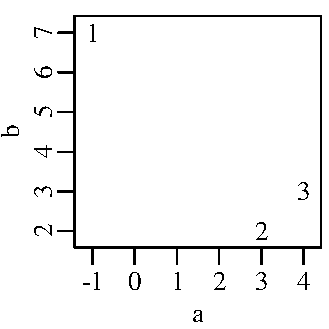
\includegraphics[width=\textwidth]{../figures/PCA2Ddata.pdf}\medskip
\end{minipage}
\begin{minipage}[t][][t]{.75\textwidth}
  \captionof{figure}{Three bivariate data points that can be
    visualised on a two-dimensional scatter plot. There is no need to
    use unsupervised learning in this case. But we will use this
    simple dataset as a toy example to understand how Principal
    Component Analysis works.\medskip}
  \label{fig:PCA2Ddata}
\end{minipage}

Imagine that you live in a one-dimensional world and cannot see the
spatial distribution of the three points represented by $X$. Then PCA
allows us to visualise the two-dimensional data as a one-dimensional
array of numbers. PCA involves the following steps\footnote{An
alternative way to find principal components is via singular value
decomposition.}
\begin{enumerate}
\item Decompose $X$ into a mean vector $M$ and a \emph{centred} data
  matrix $Y$:
  \begin{equation}
    X = 1_{3,1} M + Y =
    \left[
      \begin{array}{c}
        1 \\
        1 \\
        1
      \end{array}
      \right]
    \left[
      \begin{array}{cc}
        2 & 4
      \end{array}
      \right]
    +
    \left[
      \begin{array}{cc}
        -3 & 3 \\
        1 & -2 \\
        2 & -1
      \end{array}
      \right]
    \label{eq:XMY}
  \end{equation}

\item Compute the covariance matrix $\Sigma$ of $X$:
  \begin{equation}
    \Sigma =
    \left[
      \begin{array}{cc}
        7.0 & -6.5 \\
        -6.5 & 7.0
      \end{array}
      \right]
  \end{equation}

\item Subject $\Sigma$ to an
  \emph{eigendecomposition}, i.e. rewrite it as the product of three
  matrices:
  \begin{equation}
    \Sigma = Q \Lambda Q^{-1} =
    \left[
      \begin{array}{cc}
        0.71 & 0.71 \\
        -0.71 & 0.71
      \end{array}
      \right]
    \left[
      \begin{array}{cc}
        13.5 & 0 \\
        0 & 0.5
      \end{array}
      \right]
    \left[
      \begin{array}{cc}
        0.71 & -0.71 \\
        0.71 & 0.71
      \end{array}
      \right]
    \label{eq:eigen}
  \end{equation}

  where the diagonal elements of $\Lambda$ are called the
  \emph{eigenvalues}, and the columns of $Q$ are the
  \emph{eigenvectors}, which are also referred to as the
  \emph{loadings} in the context of PCA.

\item Define the \emph{principal components} ($P$) or \emph{scores}
  as:
  \begin{equation}
    P = Y Q = 
    \left[
      \begin{array}{cc}
        -4.24 & 0 \\
        2.12 & -0.71 \\
        2.12 & 0.71
      \end{array}
      \right]
    \label{eq:P}
  \end{equation}

\end{enumerate}

The first column of $Q$ defines the direction of maximum variance of
the bivariate dataset $X$ (direction of the line labelled PC1 in
Figure~\ref{fig:PCA2D1}).  It separates sample 1 from samples~2 and
3. Projecting the data onto this direction yields a new set of
numbers, corresponding to the first column of $P$ (PC1 in
Figure~\ref{fig:PCA2D2}). The variance of these new coordinates is
13.5, i.e. the first eigenvalue of $\Lambda$. The second column of $Q$
defines a direction that is orthogonal (perpendicular) to that defined
by the first column (direction of the line labelled PC2 in
Figure~\ref{fig:PCA2D1}). This direction accounts for the remaining
variance of the dataset, separating samples 2 and 3. Projecting the
three samples on the second principal direction yields a second set of
principal components, corresponding to the second column of $P$ (PC2
in Figure~\ref{fig:PCA2D2}). The variance of these numbers is 0.5,
i.e. the second eigenvalue of $\Lambda$.

\noindent\begin{minipage}[t][][b]{.27\textwidth}
  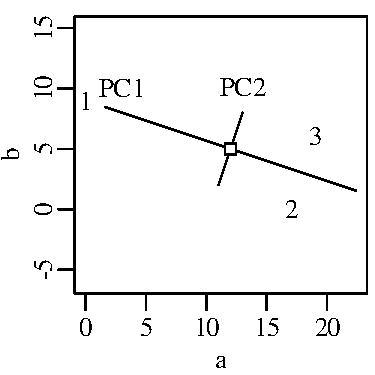
\includegraphics[width=\textwidth]{../figures/PCA2D1.pdf}\medskip
\end{minipage}
\begin{minipage}[t][][t]{.73\textwidth}
  \captionof{figure}{PCA decomposition of
    Figure~\ref{fig:PCA2Ddata}. The data $X$ are shown as numbers, $M$
    as a square, and $1_{2,1}M \pm Q \sqrt{\Lambda}$ as a cross. The
    first principal direction (running from the upper left to the
    lower right) has been stretched by a factor of $\sqrt{13.5/0.5} =
    5.2$ w.r.t the second principal direction, which runs
    perpendicular to it.\medskip}
  \label{fig:PCA2D1}
\end{minipage}

The first column of $P$ yields the desired one-dimensional
simplification of the data:

\noindent\begin{minipage}[t][][b]{.27\textwidth}
  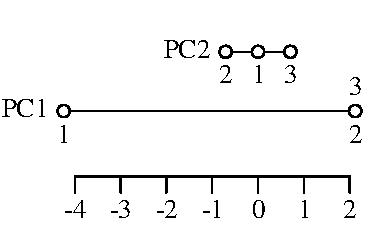
\includegraphics[width=\textwidth]{../figures/PCA2D2.pdf}\medskip
\end{minipage}
\begin{minipage}[t][][t]{.73\textwidth}
  \captionof{figure}{Projection of the three data points on the two
    principal directions yields two principal components ($P$ in
    Equation~\ref{eq:P}), representing one-dimensional representations
    of the two-dimensional data.\medskip}
  \label{fig:PCA2D2}
\end{minipage}

Using the eigenvalues $\Lambda$ in Equation~\ref{eq:eigen}, it can be
shown that the first principal component (PC1) captures
$13.5/(13.5+0.5)=96\%$ of the variance in the dataset, and the second
principal component (PC2) accounts for the remaining
$0.5/(13.5+0.5)=4\%$ of the variance. So relatively little information
is lost by discarding PC2. Then PC1 tells us that, to a first
approximation, sample~1 is very different from samples~2 and 3, which
are identical to each other. PC2 captures the remaining information,
which shows that samples~2 and 3 are, in fact, not exactly
identical. In the second principal direction, sample~1 falls in
between samples $2$ and $3$.\medskip

The scores $P$ and loadings $Q$ contain information about the samples
(1, 2 and 3) and the variables ($a$ and $b$), respectively.  We can
graphically combine all this information in a \textbf{biplot}:

\noindent\begin{minipage}[t][][b]{.25\textwidth}
  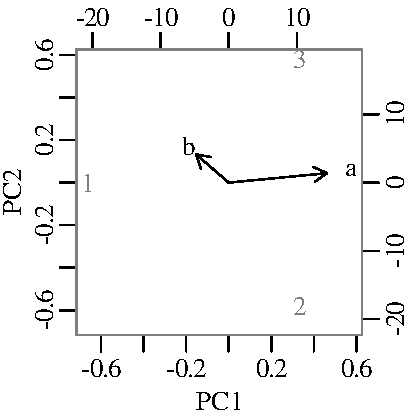
\includegraphics[width=\textwidth]{../figures/PCA2D3.pdf}\medskip
\end{minipage}
\begin{minipage}[t][][t]{.75\textwidth}
  \captionof{figure}{A biplot of both principal components along with
    the loadings of the two variables shown as arrows. The first
    principal component shows that the most important difference is
    that between sample~1 (which is rich in $b$ and poor in $a$) and
    samples 2 and 3 (which are poor in $b$ and rich in $a$). The
    second principal component captures the remaining variance, with
    sample~3 begin slightly richer in $a$ and $b$ than
    sample~2.\medskip}
  \label{fig:PCA2D3}
\end{minipage}

Although the two-dimensional example is useful for illustrative
purposes, the true value of PCA obviously lies in higher dimensional
situations. As a second example, let us consider one of \texttt{R}'s
built-in datasets:

\begingroup
\noindent\begin{minipage}[t][][b]{.55\textwidth}
\begin{tabular}{l|cccc}
      & Murder & Assault & Rape & UrbanPop \\ \hline
Alabama    &  13.2  & 236  & 21.2 & 58 \\
Alaska     &  10.0  & 263  & 44.5 & 48 \\
Arizona    &   8.1  & 294  & 31.0 & 80 \\
Arkansas    &  8.8  & 190  & 19.5 & 50 \\
California  &  9.0  & 276  & 40.6 & 91 \\
Colorado    &  7.9  & 204  & 38.7 & 78 \\
$\vdots$ & $\vdots$ & $\vdots$ & $\vdots$ & $\vdots$ \\
Wisconsin  & 2.6 & 53  & 10.8 & 66 \\
Wyoming    & 6.8 & 161 & 15.6 & 60 
\end{tabular}
\end{minipage}
\begin{minipage}[t][][t]{.45\textwidth}
  \captionof{table}{\texttt{USArrests} is a dataset that is built into
    the \texttt{R} programming environment. It contains crime
    statistics (in arrests per 100,000 residents) for murder, assault
    and rape in each of the 50 US states in 1973. Also given is the
    percentage of the population living in urban areas. Thus,
    \texttt{USArrests} is a four-column table that cannot readily be
    visualised on a two-dimensional surface.}
  \label{tab:USArrests}
\end{minipage}
\endgroup\medskip

Applying PCA to Table~\ref{tab:USArrests} yields four principal
components, the first two of which represent 62\% and 25\% of the
total variance, respectively.  Visualising the PCA results as a
biplot:

\noindent\begin{minipage}[t][][b]{.5\textwidth}
  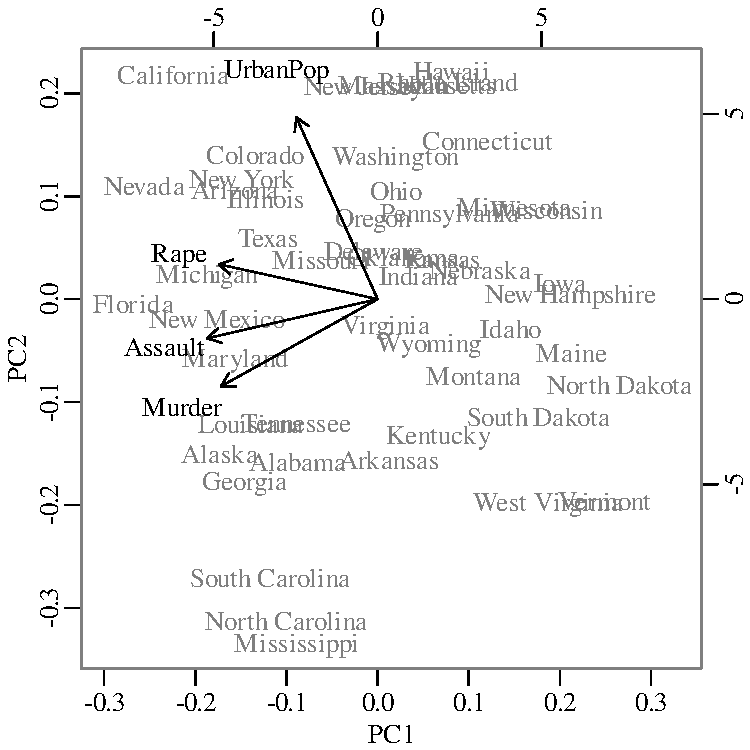
\includegraphics[width=\textwidth]{../figures/USArrests.pdf}\medskip
\end{minipage}
\begin{minipage}[t][][t]{.5\textwidth}
  \captionof{figure}{ PCA biplot of American crime statistics.  The
    grey labels mark the different states, whilst the black vectors
    mark the crimes and the percentage of the population that lives in
    urban areas. States that have a lot of crime plot on the left hand
    side of the diagram, states with little crime plot towards the
    right.  Heavily urbanised states plot at the bottom of the
    diagram, rural states plot near the top.\medskip}
  \label{fig:USArrests}
\end{minipage}

States that plot close together (such as West Virginia \& Vermont, or
Arizona \& New York, etc.)  have similar crime and urbanisation
statistics.  States that plot at opposite ends of the diagram (such as
North Dakota \& Florida, or Mississipi \& California) have contrasting
crime and/or urbanisation statistics.  The vectors for murder, assault
and rape all point in approximately the same direction, towards the
left hand side of the diagram. This tells us that the crimes are all
correlated with each other. So states that have a lot of assaults
(such as Florida), also have a lot of rape and murder. States that
plot on the right hand side of the diagram (such as North Dakota),
have low crime statistics in all categories.  The vector with the
urban population (\texttt{UrbanPop}) is perpendicular to the crime
vectors. This tells us that crime and degree of urbanisation are not
correlated in the United States.

\section{Multidimensional Scaling}
\label{sec:MDS}

Multidimensional Scaling (MDS) is a multivariate \textbf{ordination}
technique that is similar in many ways to PCA. MDS aims to extract two
(or higher) dimensional `maps' from tables of pairwise distances
between objects. Let us illustrate the method with the same synthetic
dataset of Equation~\ref{eq:X}. Using the Euclidean distance
($d[i,j]$, where $1\leq{i,j}\leq{3}$):
\begin{equation}
  d[i,j] = \sqrt{(a[i]-a[j])^2 + (b[i]-b[j])^2}
  \label{eq:euclidean}
\end{equation}

\noindent we can populate a ${3}\times{3}$ table of distances:
\begin{equation}
  d = \bbordermatrix{ & 1 & 2 & 3 \cr
    1 & 0 & 6.4 & 6.4 \cr
    2 & 6.4 & 0 & 1.4 \cr
    3 & 6.4 & 1.4 & 0
  }
  \label{eq:d}
\end{equation}

Table~\ref{eq:d} has the following properties:

\begin{enumerate}
\item{\bf symmetry}: $d[i,j]=d[j,i]$; for example, the distance from
  sample~1 to 3 equals the distance from samples~3 and 1.
\item{\bf non-negativity}: $d[i,j]\geq{0}$ and $d[i,j]=0$ if $i=j$;
  for example, the distance between sample 2 and itself is zero.
\item{\bf triangle inequality}: $d[i,j]+d[j,k]\geq{d[i,k]}$; for
  example, the sum of the distance from sample~1 to 2 and the
  distance from sample~1 to 3 is 6.4 + 6.4 = 12.8~km, which is
  greater than the distance from sample~2 to 3 (1.4).
\end{enumerate}

Given a table of this form, MDS reconstructs the original set of plot
coordinates:
\begin{equation}
  m = \bbordermatrix{ & x & y \cr
    1 & 4.24 & 0 \cr
    2 & -2.12 & -0.71 \cr
    3 & -2.12 & 0.71 
  }
  \label{eq:m}
\end{equation}

Note that Equation~\ref{eq:m} is identical to Equation~\ref{eq:P}
apart from the sign of the $x$-column.  So in this example MDS is
essentially identical to PCA. The only difference is that MDS takes a
table of distances as input, whereas PCA uses the raw data. This makes
MDS more flexible than PCA. As a second (non-trivial) example,
consider the following table of pairwise distances between European
cities:

\begin{center}
  \begin{tabular}{c|ccccccc}
  &  Athens & Barcelona & Brussels & $\ldots$ & Rome & Stockholm & Vienna \\ \hline
Athens & 0 & 3313 & 2963 & $\ldots$ & 817 & 3927 & 1991 \\
Barcelona & 3313 & 0 & 1326 & $\ldots$ & 1460 & 2868 & 1802 \\
Brussels & 2963 & 1318 & 0 & $\ldots$ & 1511 & 1616 & 1175 \\
$\vdots$ & $\vdots$ & $\vdots$ & $\vdots$ & $\ddots$ &
$\vdots$  & $\vdots$ & $\vdots$ \\
Rome & 817 & 1460 & 1511 & $\ldots$ & 0 & 2707 & 1209 \\
Stockholm & 3927 & 2868 & 1616 & $\ldots$ & 2707 & 0 & 2105 \\
Vienna & 1991 & 1802 & 1175 & $\ldots$ & 1209 & 2105 & 0 
  \end{tabular}
  \captionof{table}{Table of road distances (in km) between European
    cities. The full dataset comprises 21 cities.}
  \label{tab:eurodist}
\end{center}

Plugging this table into an MDS algorithm produces the following
output:

\noindent\begin{minipage}[t][][b]{.4\textwidth}
  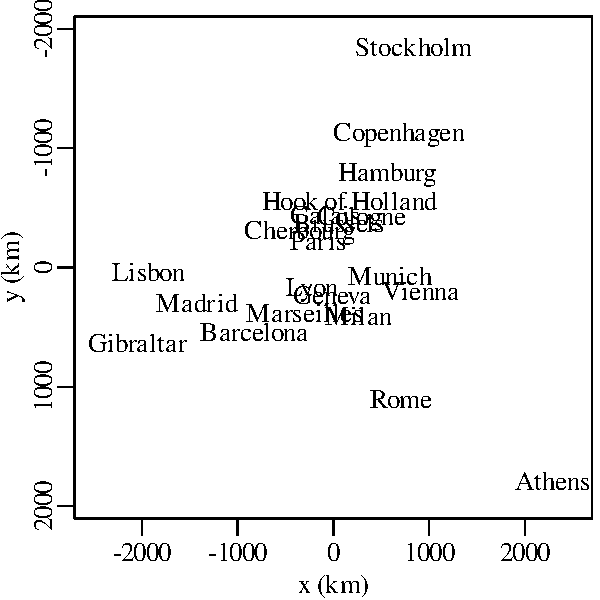
\includegraphics[width=\textwidth]{../figures/eurodist.pdf}\medskip
\end{minipage}
\begin{minipage}[t][][t]{.6\textwidth}
  \captionof{figure}{MDS configuration of the European city distance
    data (Table~\ref{tab:eurodist}). Cities (such as Lyon and Geneva)
    that are close together in the real world plot close together on
    the MDS configuration. And cities (such as Stockholm and Athens)
    that are far apart in the real world plot on opposite ends of the
    MDS configuration. But whilst the MDS configuration preserves the
    distances, it does not preserve the orientation of the cities. In
    this figure, the y-axis has been flipped, and the city locations
    are rotated $\sim 15^\circ$ in a clockwise sense compared to the
    real map of Europe.\medskip}
  \label{fig:eurodist}
\end{minipage}

We can measure the distances between the cities on the MDS map (in cm,
inches or any other unit) and plot them against the input distances
(in km) from Table~\ref{tab:eurodist}. This produces a so-called
\textbf{Shepard plot}:

\noindent\begin{minipage}[t][][b]{.3\textwidth}
  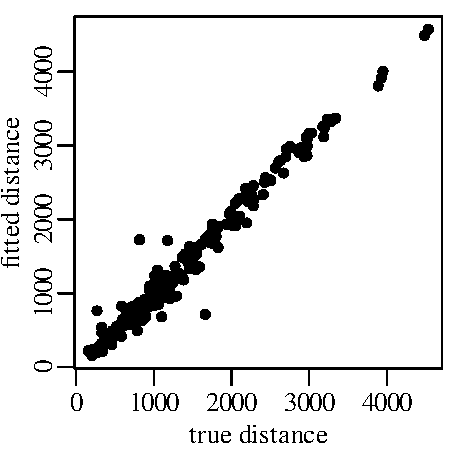
\includegraphics[width=\textwidth]{../figures/Shepard.pdf}\medskip
\end{minipage}
\begin{minipage}[t][][t]{.7\textwidth}
  \captionof{figure}{The Shepard plot of the European city distances
    shows a good agreement between the true input distances from
    Table~\ref{tab:eurodist} (x-axis) and the fitted distances
    measured on the MDS configuration of Figure~\ref{fig:eurodist}
    (y-axis). There are 21 cities in the dataset, resulting in
    $21\times{20}/2=210$ pairwise distances. Hence there are 210 data
    points on this scatter plot. Most of the scatter of the data
    around the best fit line is caused by the fact that the input data
    are \emph{road distances}, which do not perfectly agree with the
    straight line map distances.\medskip}
  \label{fig:Shepard}
\end{minipage}

The scatter of the fitted data relative to the true distances can be
quantified as the \textbf{Stress}:
\begin{equation}
  S = \sqrt{\frac{\sum_{i=1}^{n}\sum_{j=i+1}^{n}(f(d[i,j])-\delta[i,j])^2}
    {\sum_{i=1}^{n}\sum_{j=i+1}^{n}\delta[i,j]^2}}
  \label{eq:stress}
\end{equation}

\noindent where $d[i,j]$ is the input distance between objects $i$ and
$j$ (for example the Euclidean distance of Equation~\ref{eq:d}),
$\delta[i,j]$ is the fitted distance measured on the MDS
configuration, and $f$ is a monotonic transformation that essentially
maps $d[i,j]$ to the same scale as $\delta[i,j]$.  The European city
distance dataset is characterised by a Stress values of 7.5\%, which
corresponds to a `good' fit:

\begin{center}
  \begin{tabular}{c|ccccc}
    fit & poor & fair & good & excellent & perfect \\
    S & 0.2 & 0.1 & 0.05 & 0.025 & 0
  \end{tabular}
  \captionof{table}{Rule of thumb for interpreting the goodness of fit
    of an MDS configuration.}
  \label{tab:S}
\end{center}

So far we have only discussed the graphical output of MDS, but we have
not yet explained how this output is produced. It turns out that there
are several ways to do so. In its simplest form (\textbf{classical
  MDS}), the method consists of a simple sequence of matrix operations
that are similar to the PCA algorithm outlined in
Equations~\ref{eq:XMY} -- \ref{eq:P}. An alternative and more widely
used approach (\textbf{nonmetric MDS}) uses an iterative gradient
search algorithm to minimise Equation~\ref{eq:stress}.\medskip

Nonmetric MDS is more flexible than classical MDS because it
accommodates unconventional `dissimilarity' measures that do not
necessarily have to behave like conventional distances. So instead of
physical distances expressed in kilometres or miles, we can also use
MDS to interpret differences in chemical concentration, density,
degree of correlation, and many other numerical quantities. Consider,
for example, the detrital zircon U--Pb geochronology data of
Section~\ref{sec:nonparametric}. Figure~\ref{fig:KS} showed that we
can express the `dissimilarity' between two U--Pb age spectra using
the Kolmogorov-Smirnov (K-S) statistic. Repeating this exercise for a
collection of 13 samples yields a $13\times{13}$ matrix of K-S values:
\begin{equation}
  d = 
  \bbordermatrix{  & 1 & 2 & 3 & 4 & \boxed{5} &
    6 & 7 & 8 & 9 & 10 & L & T & \boxed{Y} \cr
    1 & 0 & 14 & 33 & 27 & 18 & 14 & 15 & 22 & 48 & 32 & 42 & 37 & 40 \cr
    2 & 14 & 0 & 36 & 33 & 16 & 14 & 15 & 24 & 46 & 32 & 47 & 42 & 43 \cr
    3 & 33 & 36 & 0 & 19 & 24 & 44 & 47 & 55 & 17 & 10 & 13 & 12 & 8 \cr
    4 & 27 & 33 & 19 & 0 & 20 & 38 & 41 & 48 & 28 & 14 & 21 & 17 & 16 \cr
    \boxed{5} & 18 & 16 & 24 & 20 & 0 & 22 & 24 & 33 & 31 & 20 & 33 & 28 & \boxed{30} \cr
    6 & 14 & 14 & 44 & 38 & 22 & 0 & 14 & 24 & 52 & 41 & 52 & 48 & 49 \cr
    7 & 15 & 15 & 47 & 41 & 24 & 14 & 0 & 16 & 51 & 43 & 54 & 49 & 52 \cr
    8 & 22 & 24 & 55 & 48 & 33 & 24 & 16 & 0 & 61 & 53 & 63 & 59 & 62 \cr
    9 & 48 & 46 & 17 & 28 & 31 & 52 & 51 & 61 & 0 & 20 & 22 & 18 & 16 \cr
    10 & 32 & 32 & 10 & 14 & 20 & 41 & 43 & 53 & 20 & 0 & 17 & 15 & 13 \cr
    L & 42 & 47 & 13 & 21 & 33 & 52 & 54 & 63 & 22 & 17 & 0 & 10 & 11 \cr
    T & 37 & 42 & 12 & 17 & 28 & 48 & 49 & 59 & 18 & 15 & 10 & 0 & 7 \cr
    \boxed{Y} & 40 & 43 & 8 & 16 & \boxed{30} & 49 & 52 & 62 & 16 & 13 & 11 & 7 & 0 
  }
  \label{eq:DZd}
\end{equation}

\noindent where the K-S values have been multiplied with 100 to remove
the decimal points. Square boxes mark the two samples shown in
Figure~\ref{fig:KS}. Equation~\ref{eq:DZd} is a symmetric matrix
containing positive values and a zero diagonal. Thus it fulfils all
the requirements for MDS analysis:

\noindent\begin{minipage}[t][][b]{.4\textwidth}
  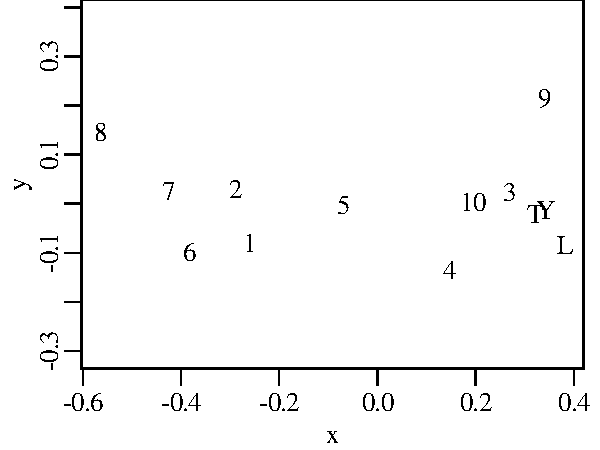
\includegraphics[width=\textwidth]{../figures/DZmds.pdf}\medskip
\end{minipage}
\begin{minipage}[t][][t]{.6\textwidth}
  \captionof{figure}{MDS configuration of the detrital zircon U--Pb
    data.  Samples that have similar age distributions (such as `Y'
    and `T') are characterised by low K-S statistics (e.g.,
    $d[Y,T]=0.07$) and plot close together. Samples that have greatly
    differing age distributions (such as `Y' and `8') are
    characterised by high K-S statistics (e.g., $d[Y,5]=0.62$) and
    plot far apart on the MDS map.\medskip}
  \label{fig:DZmds}
\end{minipage}

\section{K-means clustering}
\label{sec:kmeans}

K-means clustering is an unsupervised learning algorithm that tries to
group data based on their similarity. As the name suggests, the method
requires that we pre-specify the number of clusters ($k$) to be found
in the dataset. We will introduce this algorithm using a simple
2-dimensional dataset:

\noindent\begin{minipage}[t][][b]{.25\textwidth}
  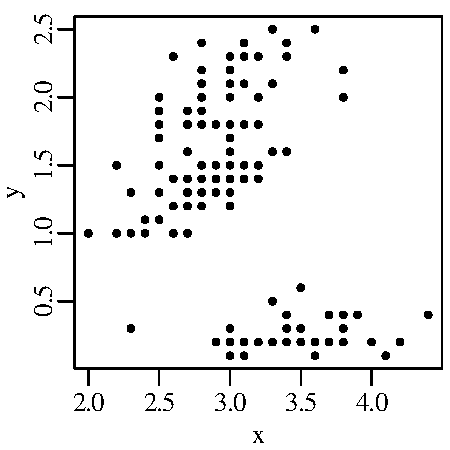
\includegraphics[width=\textwidth]{../figures/kmeans1.pdf}\medskip
\end{minipage}
\begin{minipage}[t][][t]{.75\textwidth}
  \captionof{figure}{A two-dimensional dataset to illustrate the
    k-means clustering algorithm. There are 150 data points. In this
    first exercise we will try to classify them into three groups.}
  \label{fig:kmeans1}
\end{minipage}

The k-means algorithm then proceeds as follows:

\begin{enumerate}
\item Randomly select three data points from the dataset and designate
  them as the centroids of three clusters:

  \noindent\begin{minipage}[t][][b]{.25\linewidth}
  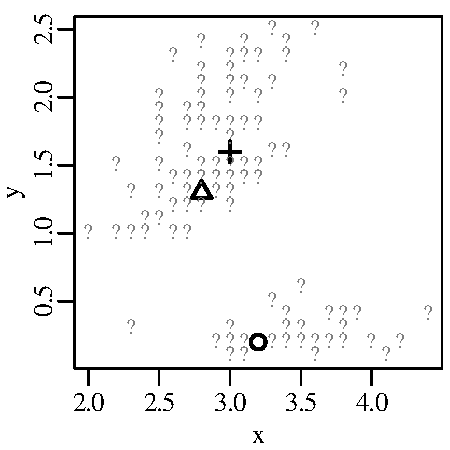
\includegraphics[width=\textwidth]{../figures/kmeans2.pdf}\medskip
  \end{minipage}
  \begin{minipage}[t][][t]{.75\linewidth}
    \captionof{figure}{Data points 48, 100 and 130 were randomly
      selected from the dataset and assigned as the centroids of
      clusters 1 (circle), 2 (triangle) and 3 (cross).}
    \label{fig:kmeans2}
  \end{minipage}
  
\item Reassign each data point to the cluster whose centroid is
  closest to it:

  \noindent\begin{minipage}[t][][b]{.25\linewidth}
  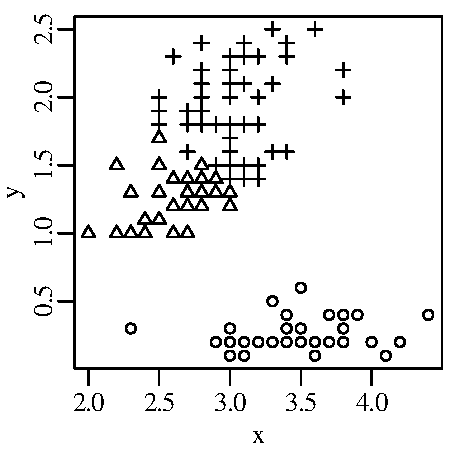
\includegraphics[width=\textwidth]{../figures/kmeans3.pdf}\medskip
  \end{minipage}
  \begin{minipage}[t][][t]{.75\linewidth}
    \captionof{figure}{Replace each of the question marks in
      Figure~\ref{fig:kmeans2} with the symbol (circle, triangle or
      cross) that is closest to it, using the Euclidean distance of
      Equation~\ref{eq:euclidean}.}
    \label{fig:kmeans3}
  \end{minipage}

\item Calculate a new centroid for each cluster:

  \noindent\begin{minipage}[t][][b]{.25\linewidth}
    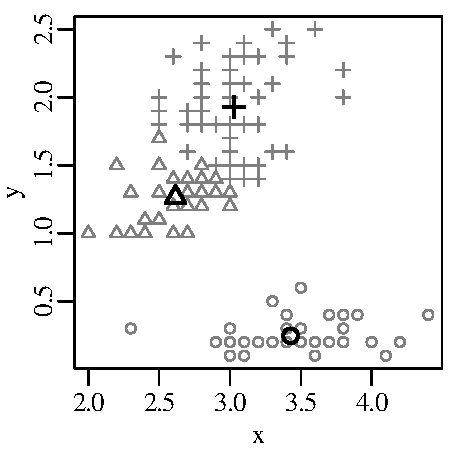
\includegraphics[width=\textwidth]{../figures/kmeans4.pdf}\medskip
  \end{minipage}
  \begin{minipage}[t][][t]{.75\linewidth}
    \captionof{figure}{The grey symbols are the same as the black
      symbols in Figure~\ref{fig:kmeans3}. The black symbols are the
      average $\{x,y\}$-positions of all the samples within each
      cluster. These are different than the previous values shown in
      Figure~\ref{fig:kmeans2}. The new values form the centroid of the
      clusters that will be used in the next iteration of the k-means
      algorithm.}
    \label{fig:kmeans4}
  \end{minipage}
  
\item Repeat steps~2 and 3 until convergence is achieved:

  \noindent\begin{minipage}[t][][b]{.25\linewidth}
  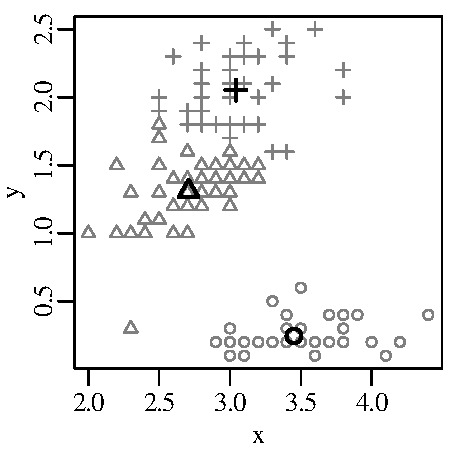
\includegraphics[width=\textwidth]{../figures/kmeans5.pdf}\medskip
  \end{minipage}
  \begin{minipage}[t][][t]{.75\linewidth}
    \captionof{figure}{Final classification of the data. Each of the
      150 data points has been assigned to one of the three clusters
      whose centroids are marked as large and bold symbols.}
    \label{fig:kmeans5}
  \end{minipage}

\end{enumerate}

The k-means algorithm can easily be generalised from two to more
dimensions because the Euclidean distance
(Equation~\ref{eq:euclidean}) can easily be generalised to any number
of dimensions.\medskip

The k-means algorithm is an unsupervised learning algorithm. This
means that it is meant to be applied to data for which we do not know
the correct classification. However, to get an idea of the success
rate of the algorithm, it is useful to apply it to a dataset for which
we do know the correct answer.  One dataset that is particularly
useful for this purpose was first introduced to statistics by
R.A. Fisher. The dataset contains the measurements in centimetres of
the sepal length and width, plus the petal length and width of 50
flowers from each of 3 species of iris:

\noindent\begin{minipage}[t][][b]{.6\textwidth}
  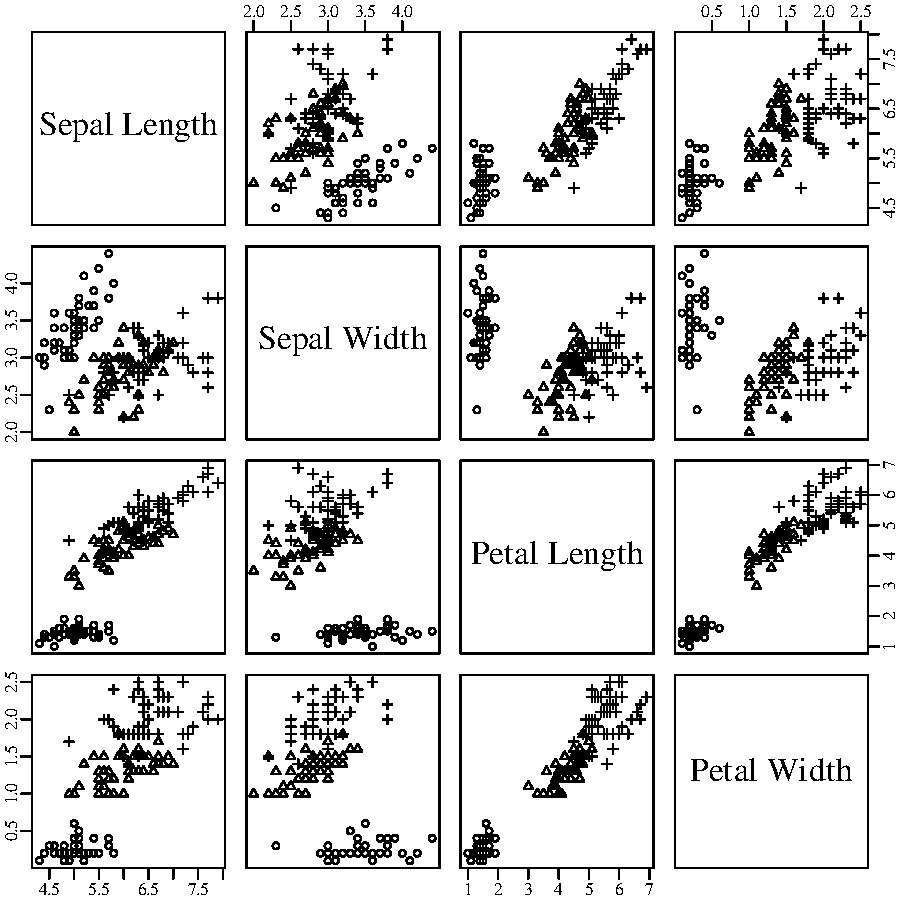
\includegraphics[width=\textwidth]{../figures/Iris.pdf}\medskip
\end{minipage}
\begin{minipage}[t][][t]{.4\textwidth}
  \captionof{figure}{Two-dimensional marginal distributions of
    R.A. Fisher's iris dataset, which comprises four variables
    measured in 150 different flowers belonging to three different
    species: \emph{setosa} (circles), \emph{versicolor} (triangles)
    and \emph{virginica} (crosses). The two-dimensional dataset of
    Figures~\ref{fig:kmeans1}--\ref{fig:kmeans5} was derived from
    panel (4,2), which sets out petal width against sepal width.  The
    classification shown in Figure~\ref{fig:kmeans5} does a decent job
    at classifying the 150 flowers into three groups but the
    classification is not perfect. For example, the flower in the
    lower left corner of panel (4,2) belongs to \emph{setosa} but was
    incorrectly classified as \emph{versicolor} in
    Figure~\ref{fig:kmeans5}.  \medskip}
  \label{fig:Iris}
\end{minipage}

For the iris dataset, we already know which species each of the 150
flowers belongs to. We can then ignore this information and apply the
k-means algorithm to the four dimensional measurements.  Afterwards,
we can compare the resulting classification to the true species and
visualise them on a $3\times{3}$ contingency table:

\begin{center}
  \begin{tabular}{c|ccc}
    cluster & setosa & versicolor & virginica \\ \hline
    1 & 50 & 0 & 0 \\
    2 & 0 & 48 & 14 \\
    3 & 0 & 2 & 36 
  \end{tabular}
  \captionof{table}{Classification results of the k-means algorithm
    applied to Fisher's iris data.}
  \label{tab:kmeansIris}
\end{center}

Table~\ref{tab:kmeansIris} shows that all flowers of the \emph{setosa}
species were collected in the same group (cluster~1). This is not
suprising when one considers that, in Figure~\ref{fig:Iris}, the
circle symbols form a distinct group in all the panels. 48 out of 50
\emph{versicolor} flowers were classified into the second cluster,
with the remaining two flowers being misclassified into the third
cluster. Finally, 36 out of 50 \emph{virginica} flowers were
classified into the third cluster, whilst 14 ended up in cluster 2.
The difficulty in separating the \emph{versicolor} and
\emph{virginica} flowers is caused by the overlap between their four
dimensional data clouds of measurements.

\section{Hierarchical clustering}
\label{sec:hierarchical}

The k-means clustering algorithm of Section~\ref{sec:kmeans} requires
that we pre-specify the number of groups.  It is not always obvious
how to choose this number, although exercise~\ref{it:ex-withinss} of
Chapter~\ref{sec:ex-unsupervised} explores a method to help pick an
optimal number of clusters.  Hierarchical clustering is an alternative
approach that builds a hierarchy from the bottom-up, and does not
require us to specify the number of groups beforehand. Let us again
use a simple 2-dimensional example to introduce the method:

\noindent\begin{minipage}[t][][b]{.25\textwidth}
  \begin{equation*}
  X =  \bbordermatrix{ & x & y \cr
      1 & 6 & 90 \cr
      2 & 91 & 43 \cr
      3 & 17 & 95 \cr
      4 & 20 & 70 \cr
      5 & 80 & 6
    }
  \end{equation*}
\end{minipage}
\begin{minipage}[t][][b]{.25\textwidth}
  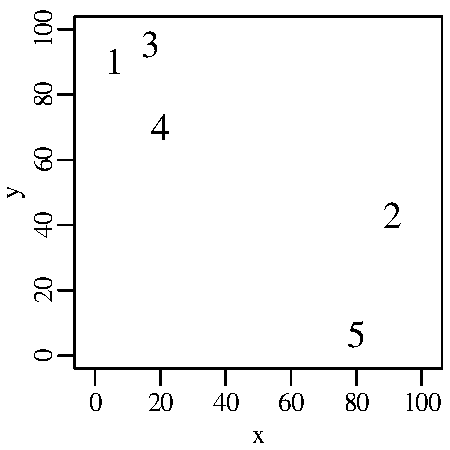
\includegraphics[width=\textwidth]{../figures/hierarchical1.pdf}\medskip
\end{minipage}
\begin{minipage}[t][][t]{.5\textwidth}
  \captionof{figure}{A simple bivariate dataset that will be used to
    illustrate the hierarchical clustering algorithm:}
  \label{fig:hierarchical1}
\end{minipage}

The algorithm works as follows:

\begin{enumerate}
\item\label{it:hierachical1} Put each data point in its own cluster
  and calculate the distances between them with
  Equation~\ref{eq:euclidean}.
  \begin{equation*}
    d = \bbordermatrix{ & 1 & 2 & 3 & 4 & 5 \cr
      1 & 0 & 97.1 & \boxed{12.1} & 24.4 & 112 \cr
      2 & 97.1 & 0 & 90.4 & 76.0 & 38.6 \cr
      3 & \boxed{12.1} & 90.4 & 0 & 25.2 & 109 \cr
      4 & 24.4 & 76.0 & 25.2 & 0 & 87.7 \cr
      5 & 112 & 38.6 & 109 & 87.7 & 0
    }
  \end{equation*}
  
\item Identify the closest two clusters (corresponding to the boxed
  numbers in step~\ref{it:hierachical1}) and join them together.

  \begin{minipage}[t][][b]{.3\linewidth}
  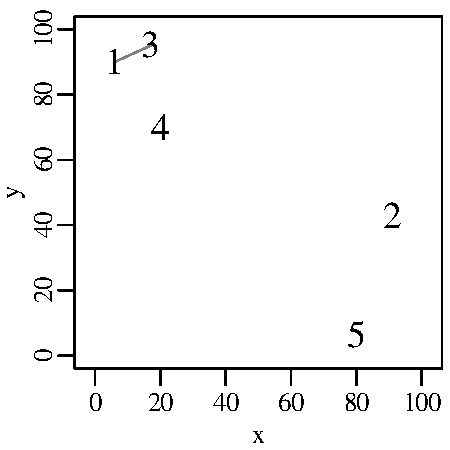
\includegraphics[width=\linewidth]{../figures/hierarchical2.pdf}\medskip
  \end{minipage}
  \begin{minipage}[t][][b]{.3\linewidth}
    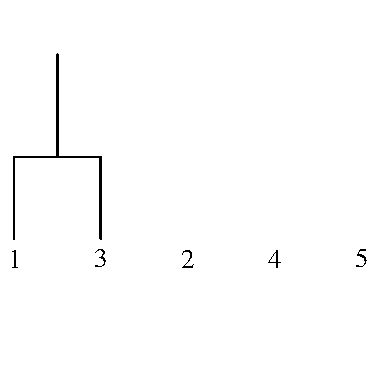
\includegraphics[width=\linewidth]{../figures/tree1.pdf}\medskip
  \end{minipage}
  \begin{minipage}[t][][b]{.4\linewidth}
  \captionof{figure}{First step of the hierarchical clustering
    process.  The closest two samples (1 and 3) have been grouped
    together into a new cluster (grey line, left). The results can
    also be visualised as a tree or \textbf{dendrogram} (right).\medskip}
  \label{fig:hierarchical2}
  \end{minipage}
  
\item\label{it:hierarchical2} Calculate the distances between the
  remaining four clusters:
  \begin{equation*}
    d = \bbordermatrix{ & 13 & 2 & 4 & 5 \cr
      13 & 0 & 97.1 & \boxed{25.2} & 112 \cr
      2 & 97.1 & 0 & 76.0 & 38.6 \cr
      4 & \boxed{25.2} & 76.0 & 0 & 87.7 \cr
      5 & 112 & 38.6 & 87.7 & 0
    }
  \end{equation*}
  \noindent where the distance between cluster~13 (which groups
  samples~1 and 3) and the other points is calculated as
  \[
  d[13,i] = \max(d[1,i],d[3,i]) \mbox{~for~}i\in\{2,4,5\}
  \]

\item Identify the closest two clusters (corresponding to the boxed
  numbers in step~\ref{it:hierarchical2}) and join them together.

  \begin{minipage}[t][][b]{.3\linewidth}
  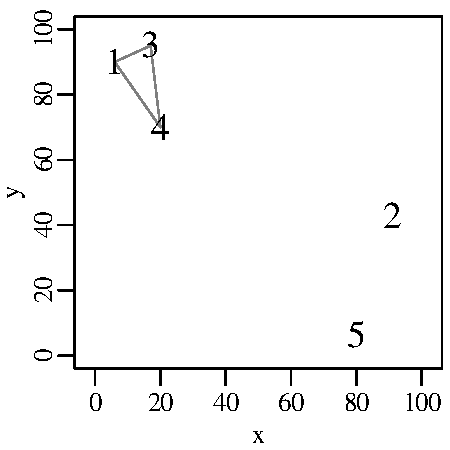
\includegraphics[width=\linewidth]{../figures/hierarchical3.pdf}\medskip
  \end{minipage}
  \begin{minipage}[t][][b]{.3\linewidth}
    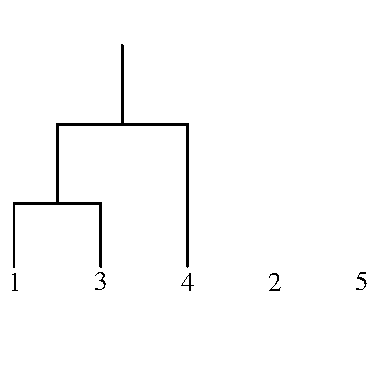
\includegraphics[width=\linewidth]{../figures/tree2.pdf}\medskip
  \end{minipage}
  \begin{minipage}[t][][b]{.4\linewidth}
  \captionof{figure}{The second step of the hierarchical clustering
    process shown as a scatter plot (left) and a dendrogram
    (right). The first order cluster is nested inside the second order
    one.\medskip}
  \label{fig:hierarchical3}
  \end{minipage}

\item\label{it:hierarchical3} Calculate the distance between the
  remaining three clusters:
  \begin{equation*}
    d = \bbordermatrix{ & 134 & 2 & 5 \cr
      134 & 0 & 97.1 & 112 \cr
      2 & 97.1 & 0 & \boxed{76.0} \cr
      5 & 112 & \boxed{76.0} & 0
    }
  \end{equation*}  
  
\item Identify the two closest clusters (corresponding to the boxed
  numbers in step~\ref{it:hierarchical3}) and join them together:

  \begin{minipage}[t][][b]{.3\linewidth}
  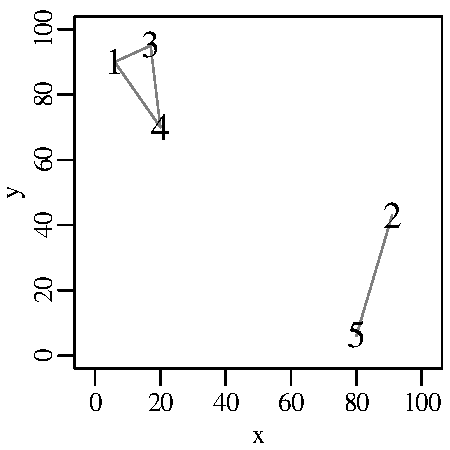
\includegraphics[width=\linewidth]{../figures/hierarchical4.pdf}\medskip
  \end{minipage}
  \begin{minipage}[t][][b]{.3\linewidth}
    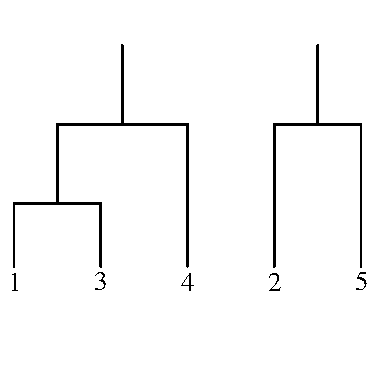
\includegraphics[width=\linewidth]{../figures/tree3.pdf}\medskip
  \end{minipage}
  \begin{minipage}[t][][b]{.4\linewidth}
  \captionof{figure}{The third step of the hierarchical clustering
    process shown as a scatter plot (left) and a dendrogram
    (right). The third cluster does not share any elements with the
    first two clusters.\medskip}
  \label{fig:hierarchical4}
  \end{minipage}

\item The final iteration yields the following tree:

  \begin{minipage}[t][][b]{.35\linewidth}
    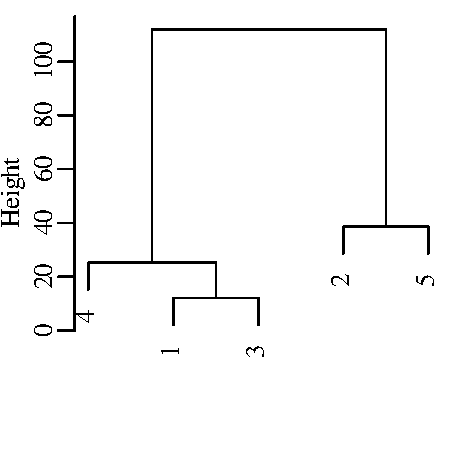
\includegraphics[width=\linewidth]{../figures/hierarchicaltree.pdf}
  \end{minipage}
  \begin{minipage}[t][][b]{.65\linewidth}
    \captionof{figure}{Final results of the hierarchical cluster
      analysis.  The tree consists of four nested clusters. The y-axis
      has units of distance: the longer the branch, the greater the
      difference between the corresponding clusters.}
  \end{minipage}
  
\end{enumerate}

Applying the same algorithm to Fisher's iris datasets produces a tree
with 150 `leaves', each corresponding to a single flower:\medskip

\noindent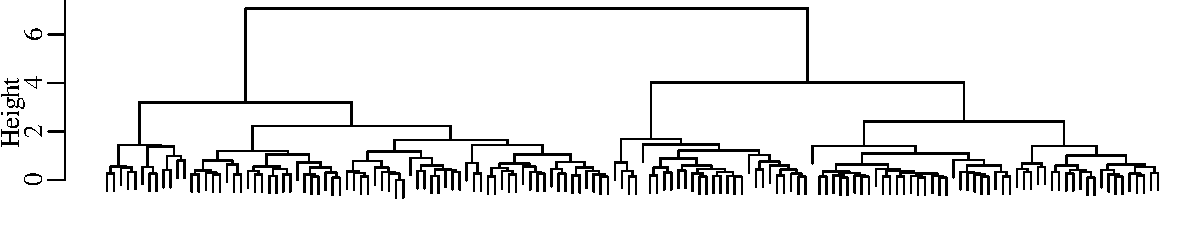
\includegraphics[width=\textwidth]{../figures/irishtree.pdf}
\begingroup \captionof{figure}{Hierarchical clustering tree of
  R.A. Fisher's iris data. Labels have been omitted to reduce
  clutter.\medskip}  \endgroup

Recall that the `height' of the tree corresponds to the maximum
possible distance between points belonging to two different clusters.
The height changes rapidly between one and three clusters, indicating
that these correspond to the most significant bifurcations. So let us
`cut down' the tree at this level:\medskip

\noindent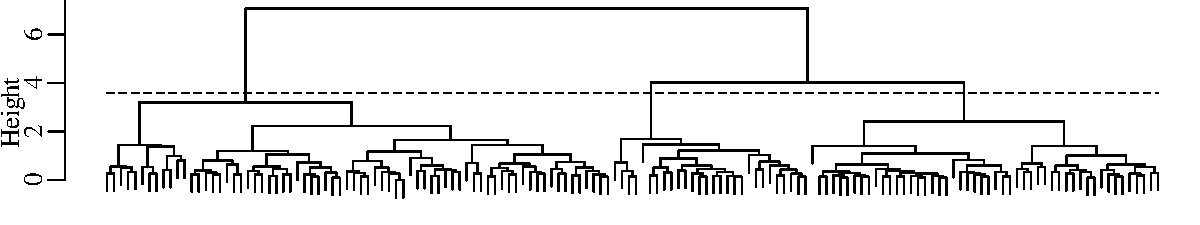
\includegraphics[width=\textwidth]{../figures/irishtreecut.pdf}
\begingroup \captionof{figure}{Cutting the tree at height=3.6 (dashed
  line) produces a simple tree with three branches, which can be used
  to classify the iris flowers into three groups.\medskip} \endgroup

Given that we know the species of all 150 iris flowers in the dataset,
we can assess the performance using a contingency table, just like
Table~\ref{tab:kmeansIris}:

\begin{center}
  \begin{tabular}{c|ccc}
    cluster & setosa & versicolor & virginica \\ \hline
    1 & 50 & 0 & 0 \\
    2 & 0 & 23 & 49 \\
    3 & 0 & 27 & 1 
  \end{tabular}
  \captionof{table}{Classification results of the hierarchical
    clustering algorithm applied to Fisher's iris data.}
  \label{tab:hclustIris}
\end{center}

The algorithm has done a good job at classifying \textit{setosa} and
\textit{virginica} but struggles with \textit{versicolor}.

